\documentclass[a4paper,12pt]{article}

%% Language and font encodings
\usepackage[english]{babel}
\usepackage[utf8x]{inputenc}
\usepackage[T1]{fontenc}

%% Sets page size and margins
\usepackage[a4paper,top=3cm,bottom=2cm,left=3cm,right=3cm,marginparwidth=1.75cm]{geometry}

%% Useful packages
\usepackage{amsmath}
\usepackage{graphicx}
\usepackage{hyperref}

\title{IGR203 project report}
\author{Alexis Bauvin -- Clément Decoodt -- Ronan Desplanques -- Ming Yang}

\begin{document}
\maketitle

\tableofcontents

\section*{Introduction}

The project we chose is the interactive restaurant menu. Indeed, this project gives us a lot of freedom of movement
in the creation of the design.

This project aims to design an interactive menu for a restaurants to be given to customers. We designed this project
with two objectives in mind : a tablet app, given to the seated client by the waiter and a smartphone app for an
outside client, wanting to order remotely.

\newpage

\section{The design}

\subsection{The overseen leads}

\subsubsection{Tablet-oriented design}

The first lead is a design thought for a tablet. It uses the whole screen estate of this platform to provide an
pleasant and original interface, while being practical. Metaphors are being used all over the design that recall
traditional restaurant menus. Furthermore, the middle of the interface gives the current state of the order by taking
the form of a restaurant table where chosen items appear on the table.

\subsubsection{Smartphone-oriented design}

This design idea relates to a smartphone implementation. On a rather small screen, it emphasises on simplicity and
clarity by using a list interface. Buttons are large and do occupy the whole screen, with greatly reduced decorative
clutter.

\subsubsection{Traditional design}

The foundation of this design is the idea to emulate as much as possible a classical menu. The main part of the
interface takes the shape of the traditional menu. It is only by touching an element that one can access extra
information and order. To increase the "paper" aspect of the interface, we recycle the characteristics of
e-readers such as curling page animations and background color.

\subsection{The chosen one}

In the end, the first design has been chosen for the main interface. It is the one to provide the most added value
against a traditional approach. Moreover, implementation-specific constraints do not look impossible to overtake.
Needs in interaction and personnalisation of the interface are answered by the design. This design is intuitive and
does not have any learning curve before being useful: tha "recognition over recall" principle is kept.

However, this design diverges from portability requirements: to be experienced to its maximum, the interface needs to
be laid out on a large screen. And by large, it is both physical size and definition. Thus, the interface needs at
least a tablet to be efficient. It is not aimed to be used by clients on their own phones.

Regarding this last point, an alternative version of the interface, more streamlined, following the second design,
will be implemented.

\subsection{Evolutions of the needs along the design}

Combining all different use needs in an unique designed proved not to be possible. The difficulty was to offer
attractive enough features to justify a swith to a fully digital menu system for on-place clients. Furthermore, it
could event be adapted to be used on the personal devices of the clients.

Our solution is to offer two interactive clients. Most of the development should be dedicated to the main tablet
interface. However, this does not results in a redundancy in the whole system because all the logic is shared between
the tablets.

\subsection{Design mechanics}

Here, we will dicuss all the details of the main chosen interface and its workings : interactions, concepts, ...

\subsubsection{Introduction screen}

The introduction screen is shown to the user at the very beginning of his interaction with the system. He is lead to
choose between "On place" or "Takeaway" to place his order. Although the default language is French, a button
looking like a flag is placed in a corner. It allows to change the language of the app.

\begin{center}
	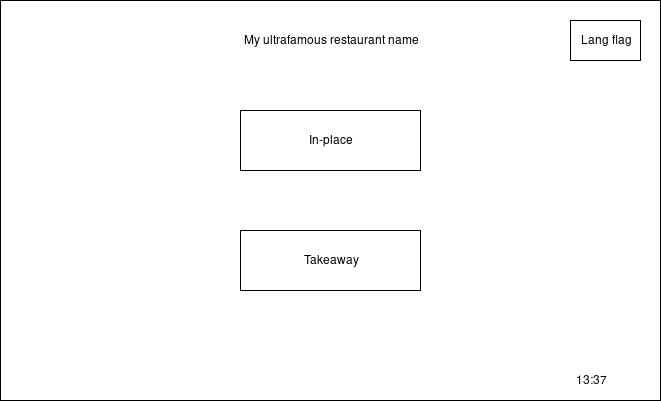
\includegraphics[width=\textwidth]{intro_screen.jpg}
\end{center}

Another layout was also considered :

\begin{center}
	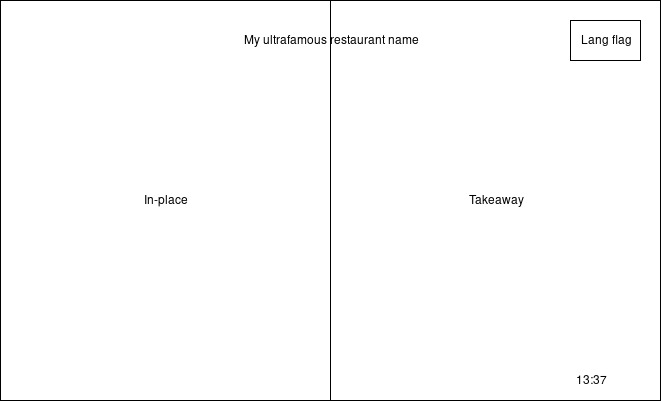
\includegraphics[width=\textwidth]{alt_intro_screen.jpg}
\end{center}

This is the final layout, as it is warmer to the user while being more efficient by reducing the precision needed to
transition to the next screen.

\subsubsection{The "on place" screen}

Cette partie de l'interface repose sur deux <<~decks~>> : l'un en bas de l'écran et l'autre à droite. Celui de droite
permet de sélectionner le sous-menu correspondant à un type d'article, par exemple plats, desserts, boissons. Celui
du bas permet de sélectionner un article au sein d'une catégorie, par exemple coq au vin, croque-monsieur. Le bouton
drapeau reste présent sur cet écran comme sur tous les autres de l'interface.

\begin{center}
	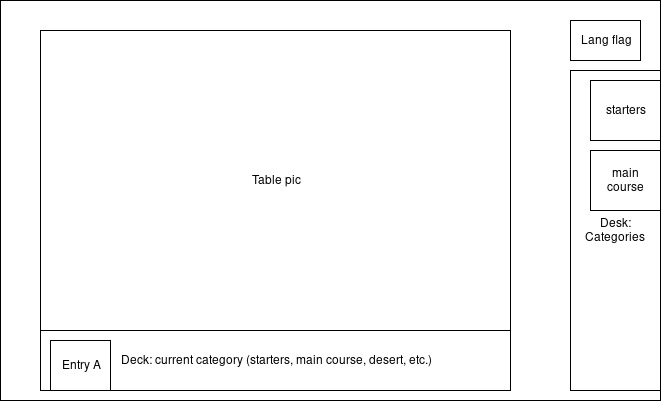
\includegraphics[width=\textwidth]{in_place_screen1.jpg}
\end{center}

Quand on clique sur un article, un écran modal s'ouvre et affiche des détails sur l'article et permet de préciser
quelques éléments (par exemple la cuisson pour une viande) avant de l'ajouter à la commande.

\begin{center}
	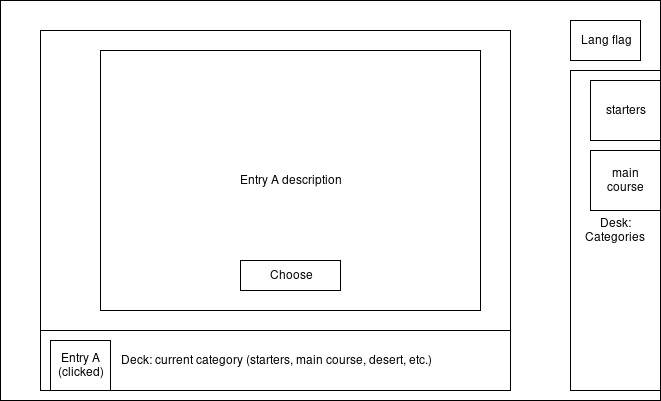
\includegraphics[width=\textwidth]{in_place_screen2.jpg}
\end{center}

La sélection se fait avec un concept de <<~deck de cartes~>> : chaque carte représente un élément, que l'on ajoute
en faisant glisser la carte. Pour sélectionner un plat dans le deck du bas, on <<~prend~>> la carte avec le doigt que
l'on <<~dépose~>> ensuite au centre de l'écran.

\begin{center}
	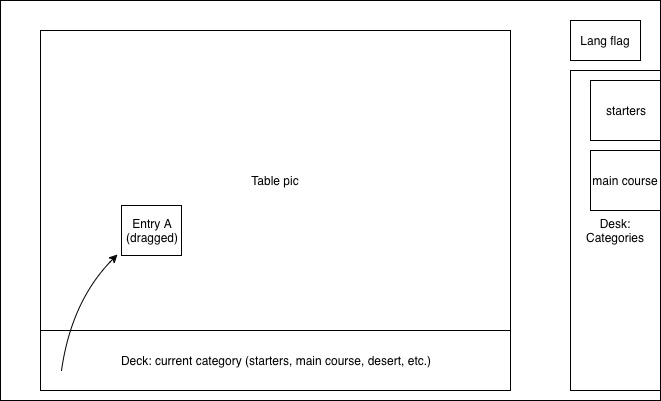
\includegraphics[width=\textwidth]{in_place_drag.jpg}
\end{center}

Le mécanisme est le même pour changer de catégorie du menu. L'on attrape une carte dans le deck de droite (par
exemple <<~entrées~>>) que l'on viens ensuite déposer sur le deck du bas, ce qui aura pour effet d'y distribuer
les cartes des nouveaux éléments.

La partie du centre de l'écran est l'image d'une table permettant de visualiser sa commande : au fur et à mesure que
l'on viens compléter sa commande, la table se garnit des éléments que l'on commande.

Le système de drag-and-drop permet d'ajouter un mécanisme de choix intuitif. Prenons l'exemple d'un steak : il est
important que le client puisse choisir la cuisson -- bien que <<~à point~>> devrait être bannie. Lorsqu'une carte
propose plusieurs choix comme ceci, des zones de surbrillance apparaissent au dessus de la table, correspondant
chacune à une option. Dans le cas de notre steak, trois zones seraient présentes : <<~saignant~>>, <<~moyen~>> et
<<~à point~>>. L'option retenue sera celle dans laquelle le client lâchera la carte.

\begin{center}
	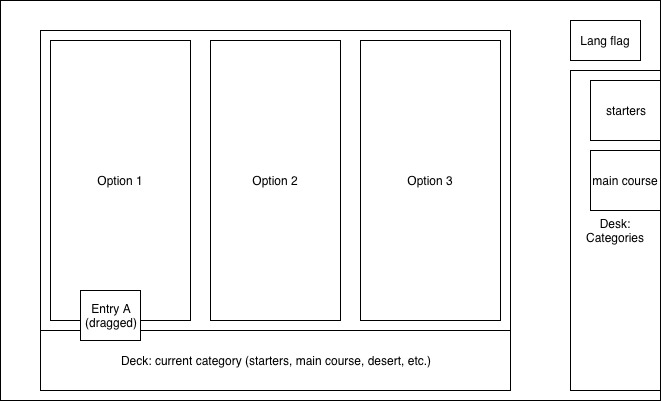
\includegraphics[width=\textwidth]{in_place_drag_options.jpg}
\end{center}

\subsubsection{The "takeaway" screen}

L'interface est plus sommaire et fonctionnelle sur cet écran~: les articles sont présentés dans une liste hiérarchisée
en sous-catégories. Le système d'écran modal du mode <<~sur place~>> est aussi présent.

\begin{center}
	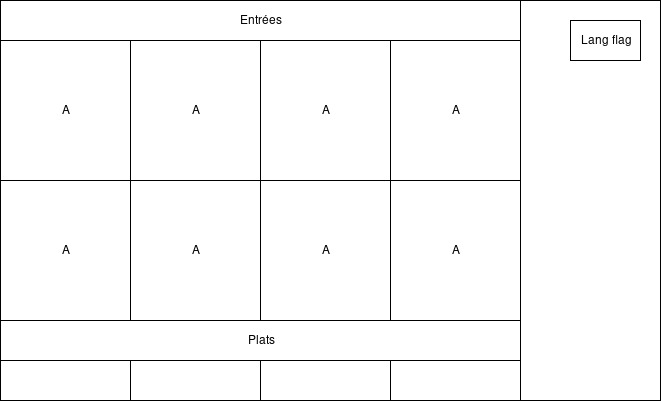
\includegraphics[width=\textwidth]{takeaway_screen.jpg}
\end{center}

\subsubsection{Confirmation screen}
Après avoir validé la commande, un écran présentant un récapitulatif de la commande invite à confirmer.

\begin{center}
	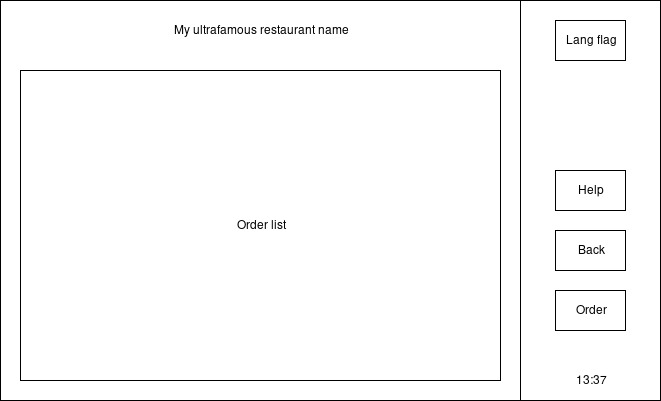
\includegraphics[width=\textwidth]{confirmation_screen.jpg}
\end{center}

\subsubsection{Final screen}

Après la validation de la commande, un écran de remerciement est affiché où l'on donne une estimation du temps
d'attente avant le service. Un champ pour fournir des informations supplémentaires au restaurant est présent.

\begin{center}
	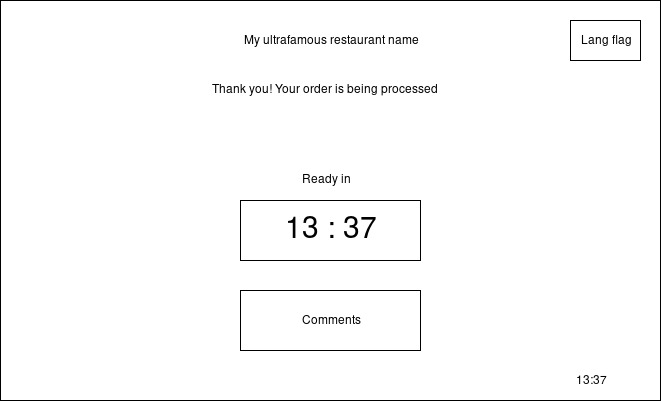
\includegraphics[width=\textwidth]{final_screen.jpg}
\end{center}

\section{Prototype}

\subsection{Practical informations}

Le prototype est hébergé sur GitHub à l'adresse suivante : \\
\url{https://github.com/friendshipismagic/pinkie-card.git}.

Ce prototype a été réalisé à l'aide du framework Qt pour plusieurs raisons. Premièrement, nous étions tous familiers
avec cet outil. De plus, comparé à iOS ou Android, c'était le seul qui n'excluait personne dans le groupe pour ne pas
posséder un iPhone ou un téléphone Android.

\subsection{Advancement}

L'avancement du prototype est facile à suive avec l'état du dépôt GitHub. Actuellement, seul l'écran d'introduction
est implémenté.

Il est important de noter que la branche la plus à jour est \texttt{develop} et non \texttt{master}.

\end{document}

